\documentclass{article}
\usepackage{graphicx}
\usepackage[utf8]{inputenc}
\usepackage{amsmath}
\usepackage{amssymb}
\usepackage{graphicx}
\usepackage{epstopdf}
\usepackage{inputenc}
\usepackage{latexsym}
\usepackage{setspace}
\usepackage{caption}
\usepackage{authblk}
\usepackage{float}
\setlength\parindent{24pt}
\usepackage[export]{adjustbox}
\usepackage{wrapfig}
\usepackage{subfig}



\begin{document}

\title{Scanning Tunneling Microscopy}
\author{Loïc James McKeever}
\affil{Mackenzie Levangie}

\maketitle

\section{Introduction}

The objective of this lab is to determine the lattice constant and unit cell configuration of a graphite sample using a scanning tunneling microscope(STM).  This will be done using tungsten tips we made ourselves as well as the image analysis software Gwyddion to study the STM images obtained.  Given the fact that the sample is graphite we expect to find a lattice constant of $a=2.46$ {\AA} and a reciprocal lattice constant of $\frac{4\pi}{a\sqrt{3}}=2.95$ {\AA} with a hexagonal crystal structure$^{[1]}$.  


\section{Materials and Methods}

In this experiment we will obtain atomic resolution images of a graphite sample.  This will be done using a Nanosurf NaoiSTM and tungsten tips made as in Figure 1. 

\begin{figure}[H]
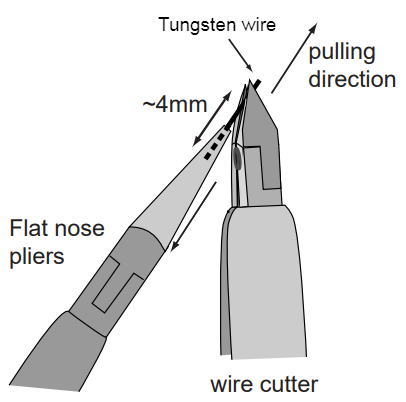
\includegraphics[scale=.4,center]{TipMaking.png}
\caption{Method used to make the tungsten tips as suggested by [2].}
\end{figure}

The PID parameters for the Z-controller were set as follows; Setpoint = 1 n{\AA}, P-Gain = 1000, I-Gain = 2000 and D-Gain = 0.  The tip bias voltage was 50 mV and we started with a scale of 500 nm.  Several images were made at a variety of scales and analyzed using Gwyddion to determine the lattice constant and the reciprocal lattice constant, by performing an ACF(Autocorrelation Function) and FFT on the image respectively.

The principle behind the Scanning Tunneling Microscope is rooted in the quantum mechanical nature of electrons. When a conductive tip is sufficiently close to a material a certain number of electrons can tunnel through the vacuum into the tip.  This then creates a tunneling current.  This current depends on the proximity of the tip to the surface of the material and can be kept constant by varying the tip to surface distance, as seen in Figure 2, and thus the topology of said surface can be mapped out.$^{[3]}$  With a sufficiently thin tip, ideally a single atom, this allows for extremely good resolution even to atomic levels. 

\begin{figure}[H]
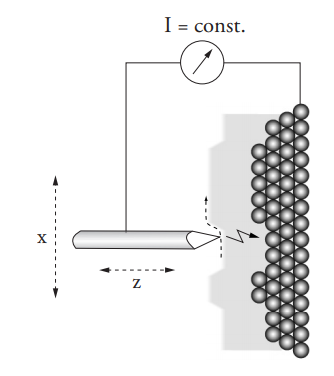
\includegraphics[scale=.7,center]{STMDiagram.PNG}
\caption{Diagram showing the theory behind the operation of the STM$^{[2]}$.}
\end{figure}


\section{Results}

We started by imaging a 500nm by 500nm section of our sample as seen in Figure 3.  This was done both to make sure our tip was suitable and to find a smooth enough section of our sample to zoom in on.

\begin{figure}[H]
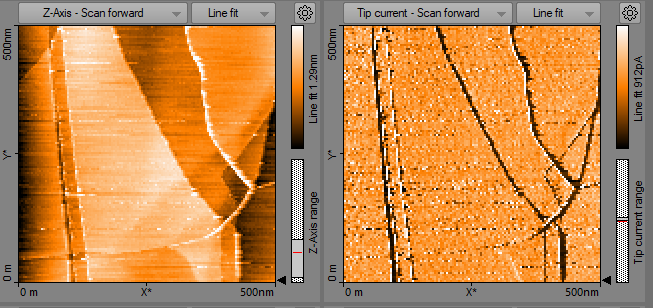
\includegraphics[scale=.7,center]{STM500nm2.PNG}
\caption{STM image of a 500 nm by 500 nm section of our sample.  On the right we see the tip z position versus it's x-y position and on the left we have the tip current versus the x-y position.}
\end{figure}

We then zoomed in to suitable 57.6 nm by 57.6 nm section as we can see in Figure 4.  A pattern is partially visible but it becomes clearly visible when we zoom in to two different 5.63 nm by 5.63nm sections as we can see in Figures 5 and 6.  We continued to zoom in to various length scales to demonstrate that the images behave as expected(the pattern becomes larger the more we zoom in) and are not just noise.  Figure 7 is a 1.54 nm by 1.54 nm section and Figure 8 is a 769 pm by 769 pm section. The hexagonal pattern acts as expected so we know this is the atomic structure of the sample and not just noise.  

\begin{figure}[H]
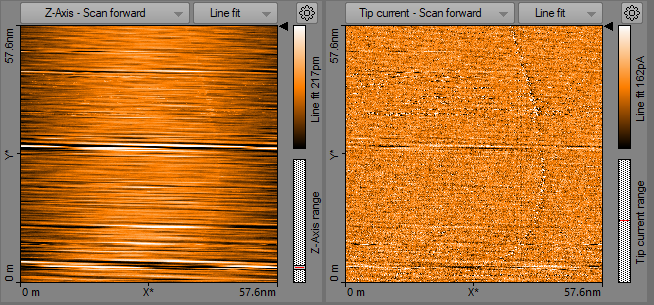
\includegraphics[scale=.7,center]{STM57d6nm2.PNG}
\caption{STM image of a 57.6 nm by 57.6 nm section of our sample.  On the right we see the tip z position versus it's x-y position and on the left we have the tip current versus the x-y position. An underlying pattern can be vaguely made out.}
\end{figure}

\begin{figure}[H]
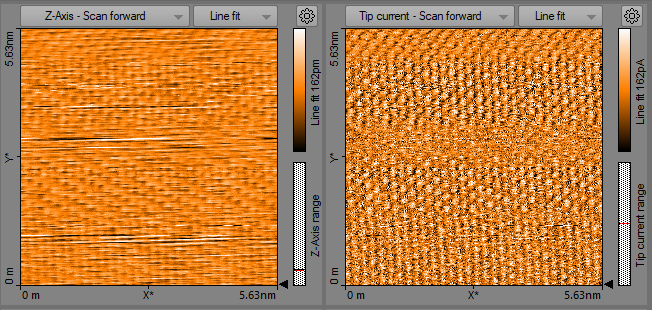
\includegraphics[scale=.8,center]{STM5d63nm2.PNG}
\caption{STM image of a 5.63 nm by 5.63 nm section of our sample.  On the right we see the tip z position versus it's x-y position and on the left we have the tip current versus the x-y position.}
\end{figure}

\begin{figure}[H]
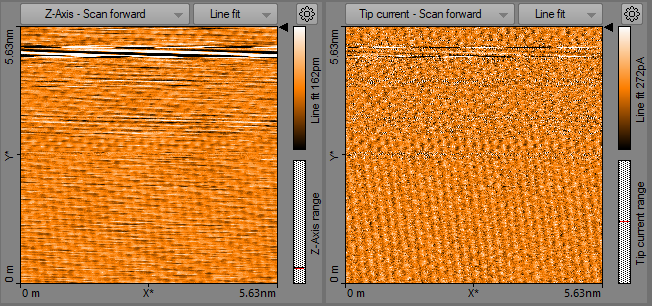
\includegraphics[scale=.8,center]{STM5d63nm22.PNG}
\caption{STM image of a 5.63 nm by 5.63 nm section of our sample.  On the right we see the tip z position versus it's x-y position and on the left we have the tip current versus the x-y position.  The atomic structure can clearly be made out and appears to be hexagonal.}
\end{figure}

\begin{figure}[H]
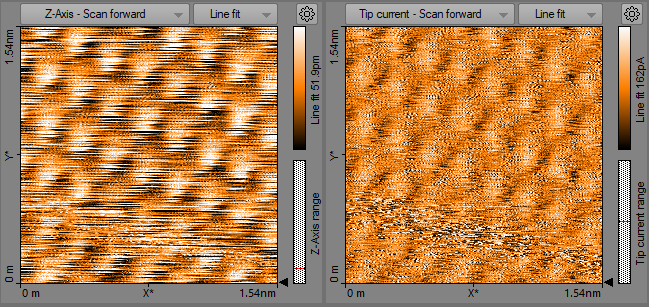
\includegraphics[scale=.8,center]{STM1d54nm2.PNG}
\caption{STM image of a 1.54 nm by 1.54 nm section of our sample.  On the right we see the tip z position versus it's x-y position and on the left we have the tip current versus the x-y position.  The pattern becomes larger as expected confirming it's not just noise.}
\end{figure}

\begin{figure}[H]
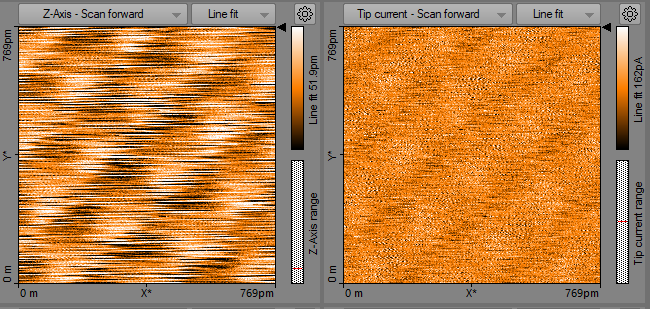
\includegraphics[scale=.8,center]{STM769Pm2.PNG}
\caption{STM image of a 769 pm by 769 pm section of our sample.  On the right we see the tip z position versus it's x-y position and on the left we have the tip current versus the x-y position.}
\end{figure}


\newpage

We chose to use the image from Figure 5 to determine the lattice constant and reciprocal lattice constants in Gwyddion.  Figure 9 shows the lattice constant determined after the data had undergone ACF, we find $a$ somewhere between $2.144$ {\AA} and $2.534$ {\AA}.  Figure 10 shows the reciprocal lattice constant determined after the data had undergone FFT, we find $\frac{4\pi}{a\sqrt{3}}$ somewhere between $2.693$ {\AA} and $3.003$ {\AA}.  

\begin{figure}[H]
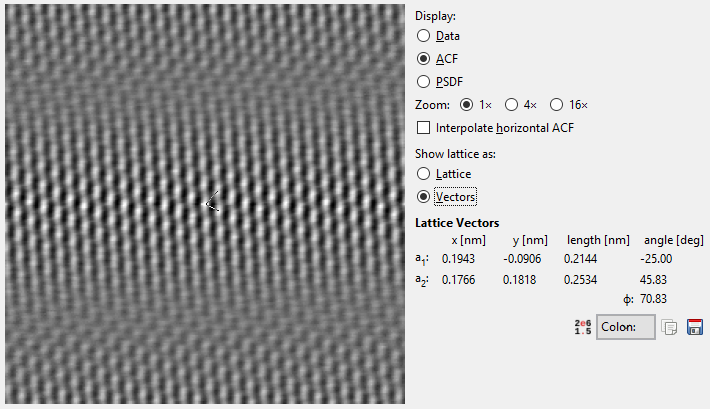
\includegraphics[scale=.8,center]{STMLatticeACF.PNG}
\caption{Lattice measurement of STM image done in Gwyddion.  The data has been processed using ACF.  The lattice constant is measured to be between $2.144$ {\AA} and $2.534$ {\AA}.}
\end{figure}

\begin{figure}[H]
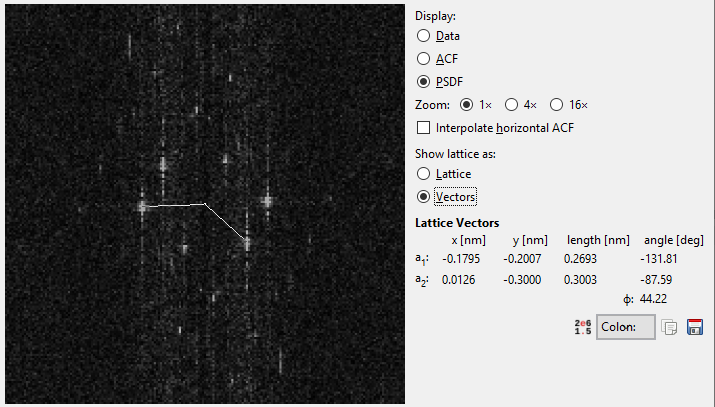
\includegraphics[scale=.8,center]{STMLatticeFFT.PNG}
\caption{Lattice measurement of STM image done in Gwyddion.  The data has been processed using FFT.  The lattice constant is measured to be between $2.693$ {\AA} and $3.003$ {\AA}.  We should also note that the hexagonal structure is much more clear after the FFT.}
\end{figure}

Finally we captured the I-V curve for graphite between -1.5V and 1.5V.  Taking the derivative of this curve gives us the LDOS(Local Density Of States) for that particular position on the sample.$^{[4]}$  This should be different at different points because of the structure, points above an atom should have a higher density of states than points in the middle of the hexagonal structure since the electrons are more likely to be found around the atoms.  Figures 11 and 12 should the I-V curve and it's derivative at two different points of the sample.

\begin{figure}[H]
    \subfloat[This chart shows the I-V curve taken at a point (20.3 nm, -23.9nm).]{{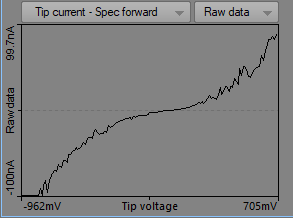
\includegraphics[scale=.8]{STMIVRAWP1.PNG} }}
    \qquad
    \subfloat[This chart shows the derived data from the first chart and gives the LDOS at this point.]{{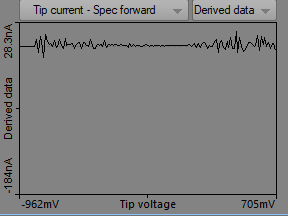
\includegraphics[scale=.8]{STMIVDERP1.PNG} }}
    \caption{Raw and derived I-V data at point 1.}
    \label{fig:example}
\end{figure}

\begin{figure}[H]
    \subfloat[This chart shows the I-V curve taken at a point (17.5 nm, -21.8nm).]{{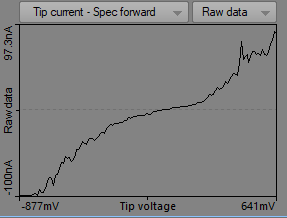
\includegraphics[scale=.8]{STMIVRAWP2.PNG} }}
    \qquad
    \subfloat[This chart shows the derived data from the first chart and gives the LDOS at this point.]{{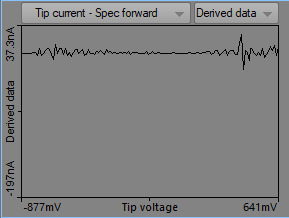
\includegraphics[scale=.8]{STMIVDERP2.PNG} }}
    \caption{Raw and derived I-V data at point 2.}
    \label{fig:example}
\end{figure}

\section{Discussion}

The STM images we took of our graphite sample showed a consistent hexagonal pattern that behaved as expected under various length scales which confirms that it is the atomic structure of the graphite and not just noise.  We were able to determine the lattice constant of our pattern using ACF and FFT on our data in Gwyddion.  This gave us a range between $2.144$ {\AA} and $2.534$ {\AA} for our lattice constant $a$ and between $2.693$ {\AA} and $3.003$ {\AA} for our reciprocal lattice constant $\frac{4\pi}{a\sqrt{3}}$.  These results are consistent given that we expected $a=2.46$ {\AA} and $\frac{4\pi}{a\sqrt{3}}=2.95$ {\AA}.  We can see though that in Figure 10 the hexagon is not regular as expected but is slightly slanted.  This could be due to a slight slope on our z axis when we took the image.  In the future we should correct for that slope more effectively. As expected the derivative of the I-V curve, which gives the local density of states, was different at two different positions.
There are a few things that effect the atomic scale image quality. The scan range;  too large and the structure is too small to see but too small and the structure loses its sharpness.  The time per scan line;  too fast and you lose precision since the tip's z-position is changed constantly and needs to react to the change in the tunneling current.  The the bias voltage determines how close the tip gets to the sample;  too low of a voltage and you end up too far away from the sample giving you a weak tunneling current but too high of a voltage and you get too close and risk scraping the sample which would ruin the image.  The tunneling current;  the weaker the tunneling current the smaller the changes in the tip's z-position which will give a very low resolution image.

\section{Conclusion}

In conclusion we were able to determine the lattice constant of our graphite sample, which has a hexagonal lattice pattern, to be  between $2.144$ {\AA} and $2.534$ {\AA} which is consistent with the expected value of $a=2.46$ {\AA}.  This was confirmed by doing a FFT on our image giving us a reciprocal hexagonal lattice with a lattice constant between $2.693$ {\AA} and $3.003$ {\AA} which is consistent with the expected value of $\frac{4\pi}{a\sqrt{3}}=2.95$ {\AA}.   

\section{References}

 [1] Crystal Structure of Graphite, Graphene and Silicon, Dodd Gray, Adam McCaughan, Bhaskar Mookerji, Physics for Solid State Applications, March 2009


\noindent [2] Nanosurf NaioSTM Operating Instructions for Naio Control Software Version 3.1

\noindent [3] Theory of the scanning tunneling microscope, J. Tersoff and D. R. Hamann, Physical Review B Volume 31, Number 2 January 1985

\noindent [4] Introduction to Scanning Tunneling Microscopy, C. Julian Chen, Oxford University Press, 1993


\end{document}
